\documentclass[11pt,letterpaper]{article}

\usepackage[letterpaper,margin=0.8in,nohead]{geometry}

\usepackage[colorlinks]{hyperref}
\usepackage{url}
\usepackage{breakurl}

\hypersetup{
    colorlinks,
    linkcolor={red},
    citecolor={red},
    urlcolor={blue}
}

\usepackage{verbatim}
\usepackage{fancyvrb}
\usepackage{scrextend}
\usepackage{enumitem}
\usepackage{url}
\usepackage{subcaption}
\usepackage[dvipsnames]{xcolor}

\usepackage{filecontents}
%\usepackage{natbib}
%\nobibliography*

\usepackage{caption}
\usepackage{graphicx}

\usepackage{changepage}   % for the adjustwidth environment

\newenvironment{answer}{\em \color{blue} \begin{adjustwidth}{1cm}{1cm}}{\end{adjustwidth}}

% math
\usepackage{amsthm,amsmath}
\usepackage{amsfonts}

\newcommand{\mc}[1]{\mathcal{#1}}	% Mechanisms / Algorithms
\newcommand{\rv}[1]{\mathbf{#1}}    % Random variable

\newcommand{\pr}[1]{\mathrm{Pr}\{#1\}} % Probability

\newtheorem{corollary}{\bf Corollary}%[theorem]
\newtheorem{lemma}{\bf Lemma}%[theorem]
\newtheorem{definition}{\bf Definition}%[section]

\newtheorem{observation}{\bf Observation}%[theorem]



% load cleveref last!
\usepackage[capitalise]{cleveref}

\crefname{observation}{Observation}{Observations}


\begin{document}

\title{\vspace{-20mm} EN3240: Embedded Systems Engineering \\Assignment 2 --- IoT Project}

%% This is an individual assignment!!
%% TODO: put your name and index number here!
\author{Name: Thalagala B. P. \\ Index No: 180631J}

\maketitle

\begin{center}
	\color{red}\bf This is an individual assignment! \\ Due Date: 25 September 2022 by 11.59 PM
\end{center}

\section*{Instructions}
%

Follow the steps given below.
Submit the node-red flow as XXXXX.json and Arduino code as XXXXX.ino to Moodle, where XXXXX is your index number. This assignment accounts for 20\% of your final grade.

%%%%%%%%%%%%%%%%%%%%%%%%%%%%%%%%%
%%%%%%%%%%%%%%%%%%%%%%%%%%%%%%%%%

\subsection*{Part I:  Weather Application (12 marks)}

Build a node-red application to get the weather data in an user-provided location from OpenWeather (A sample of the Dashboard is shown in Figure~\ref{fig:nodered-dashboard-samples}). It should have the following features:

\begin{itemize}
    \item The dashboard should have three main tabs: 
        \begin{enumerate}
            \item \textcolor{NavyBlue}{Weather}
            \item \textcolor{magenta}{Charts}
            \item \textcolor{ForestGreen}{Settings}
        \end{enumerate}
    
    \item \textcolor{NavyBlue}{Weather Tab} 
    
    \begin{enumerate}
        \item The user should be able to enter the location as i) coordinates or ii) city and country through a text field(s) and submit.
        
        \item The title of the description section should be the location entered by the user. If coordinates are used to specify the location, retrieve the city using OpenWeather.
        
         \item Show temperature, humidity, pressure, wind speed, wind direction, sunrise time, sun setting time of the current day. These data should be updated every 30s by default.
         
        \item Use suitable customized gauges for the above parameters (e.g., a compass for wind direction). 
        
        \item There should be a speaker icon, which, when clicked, would enable the user to hear the description of the weather. 
        
        \item There should be a warning limit for a selected parameter (e.g., temperature, pressure, ...). Use a dropdown list to choose the parameter and a slider to set the limit. (e.g., $ 25^\circ C $ for temperature, 30 km for wind, etc.). When this limit is exceeded, a notification should appear as a warning displaying the current value of the parameter (e.g., Warning! Temperature is $ 30^\circ C $. Exceeds the limit by $ 5^\circ C $) 
        
    \end{enumerate}
    
    \item \textcolor{magenta}{Charts Tab} 
    
    \begin{enumerate}
        \item There should be charts that show the temperature, humidity, wind speed of the past hour.
    \end{enumerate}
    
    \item \textcolor{ForestGreen}{Settings Tab} 
    
    \begin{enumerate}
       
        \item The user should be able to select whether the location is entered as i) coordinates or ii) city and country.
    
        
        \item  The user should be able to change the refresh time (use numeric palette).
    
        \item Use a switch to turn the charts feature on and off.
    
    \end{enumerate}
    

\end{itemize}

\noindent Expected three tabs of the dashboard are illustrated in Figure~\ref{fig:nodered-dashboard-samples}. \textbf{Submit the node-red flow to Moodle}. 

\subsection*{Part II: Weather Warning Device (8 marks)}

Extend your Weather Application to include a Weather Warning Device implemented with the NodeMCU. Link the above application to your NodeMCU via MQTT. The complete system is illustrated in Figure~\ref{fig:node-mcu-weather-integration}.

\begin{itemize}
    \item Blink the built-in LED of the node-MCU in a warning situation. The threshold/limit for the warning situation is set as described in Part I.
    \item Change the blinking interval from 5s to 500ms according to the exceeded amount. For an example, 5s interval if the value is just above the warning limit and decreasing up to 500ms interval if it reaches a maximum value. You may decide what the maximum value is.
    \item Use test.mosquitto.org/ as the MQTT broker.
\end{itemize}

\noindent \textbf{Submit the resulting Arduino code to Moodle} after verifying that it works properly with the hardware.

\begin{figure}[h]
    \centering
    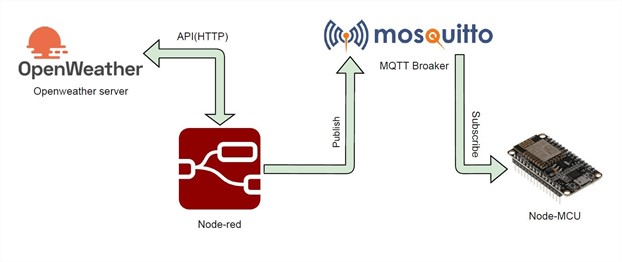
\includegraphics[width=1\columnwidth]{images/assign2-node-mcu-weather-integration.jpg}
    \caption{Overview of different components.} \label{fig:node-mcu-weather-integration}
\end{figure}

\subsection*{Useful Links}
\begin{itemize}
    \item A demo of the dashboard can be found \href{https://dms.uom.lk/s/yxnzNfEZcHHqRmo}{here}.
    \item An overview of the weather API can be found \href{https://dms.uom.lk/s/iQTGPT7eNDKoJYy}{here}. 
    \item A NodeMCU Simulator can be found here \href{https://wokwi.com/projects/322410731508073042}{here}. (If you are unable to find a NodeMCU)
\end{itemize}

 




\newpage

\begin{minipage}{\linewidth}% to keep image and caption on one page
\makebox[\linewidth]{%        to center the image
  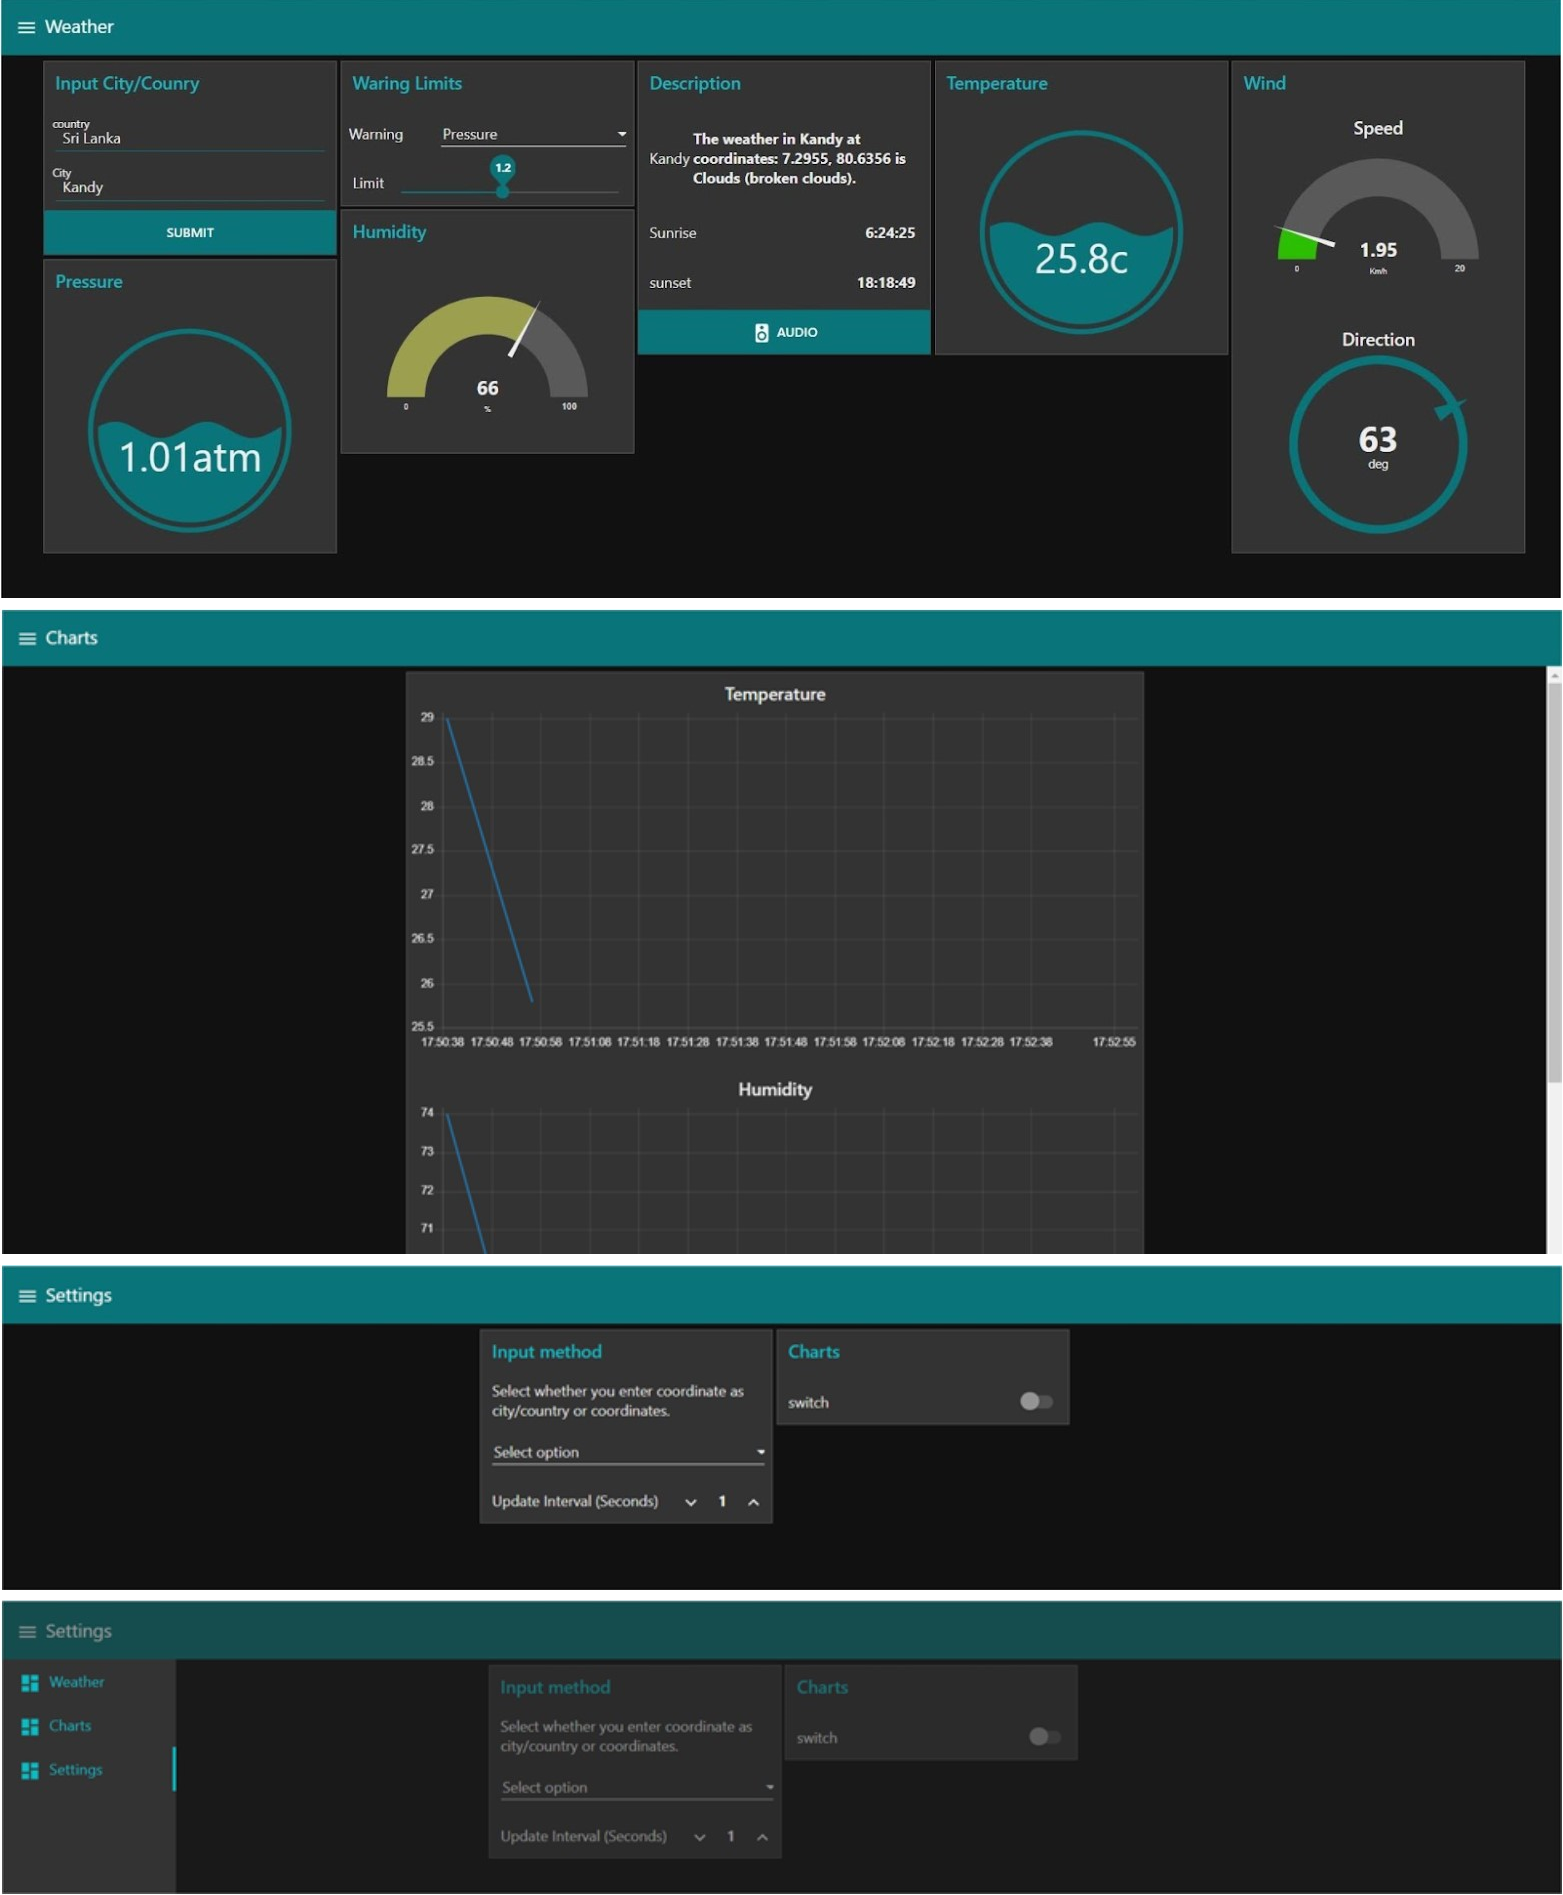
\includegraphics[keepaspectratio=true,scale=0.45]{images/assign2-nodered-dashboard-samples.png}}
\captionof{figure}{Expected three tabs of the dashboard.}\label{fig:nodered-dashboard-samples}%      only if needed  
\end{minipage}

\newpage



\end{document}
